
\chapter{Radiance Fields}
\label{chapter:nerfs}


\section{Introduction}

%Remnind the reader about the plenoptic function and lightfields. 

In this chapter we will come full circle. Starting from the Greek's model of optics (\chap{\ref{chap:challenge_of_vision}}) that postulated that light is emitted by the eyes and travels in straight lines, touching objects in order to produce the sensation of sight (extramission theory), radiance fields will use that analogy to model scenes from multiple images. Here, geometry-based vision and machine learning will meet. 

Before diving into radiance fields, we will review two relevant concepts, Adelson and Bergen's \index{Plenoptic function}\textbf{plenoptic function} and Kajiya's \index{Rendering equation}\textbf{rendering equation}.

\subsection{The Plenoptic Function}

We first discussed the plenoptic function when we introduced the challenge of vision in \chap{\ref{chap:challenge_of_vision}}.
\index{Plenoptic function}

As stated in the work by Adelson and Bergen \cite{Adelson91}, the plenoptic function tries to answer the following question: ``We begin by asking what can potentially be seen. What
information about the world is contained in the light
filling a region of space?''


Given a scene, the plenoptic function is a full description of all the light rays that travel across the space (\fig{\ref{fig:nerfs:plenoptic_function}}). The plenoptic function tells us the light intensity of a light ray passing through the 3D point $(X, Y, Z)$ from the direction given by the angles $(\psi, \phi)$, with wavelength $(\lambda)$, at time $t$:
\begin{equation}
\lightfield (X, Y, Z, \psi, \phi, \lambda, t)
\end{equation}
In this chapter we will ignore time and we will only use three color channels instead of the continuous wavelength. We can represent the plenoptic function with the parametric form $\lightfield_{\theta}$ where the parameters $\theta$ have to be adapted to represent each scene. 

\begin{figure}[t]
    \centerline{
    \includegraphics[width=1\linewidth]{figures/nerfs/plenoptic_function.eps}
    }
    \caption{Plenoptic function \cite{Adelson91}. 
    The figure shows a slice of the plenoptic function at four locations. Two of the locations are in free space, and two other locations are inside a pinhole camera.}
    \label{fig:nerfs:plenoptic_function}
\end{figure}

%L7d=P(x,y,z,θ,ϕ,t,λ),

An image gets formed by summing all the light rays that reach each sensor on the camera (which is a section of the plenoptic function).  \Fig{\ref{fig:nerfs:plenoptic_function}} shows an illustration of the plenoptic function at four points, two of them are inside a pinhole camera and are used to form an image of what is outside. The plenoptic function inside the pinhole camera has most of the values set to zero and only specific directions at each location have non-zero values. 

In \chap{\ref{chap:challenge_of_vision}} we discarded the plenoptic function by simply saying, ``Although recovering the entire plenoptic function would have many applications, fortunately, the goal of vision is not to recover this function.'' But we did not really give any argument as to why simplifying the goal of vision was a good idea. What if we now we change our minds and decide that one useful goal of vision is to actually recover that function entirely? Can it be done? How?

If we had access to the plenoptic function of a scene, we would be able to render images from all possible viewpoints within that scene. One example is lumigraph \index{Lumigraph}{\bf lumigraph} \cite{Gortler1996} which extracts a subset of the plenoptic function from a large set of images showing different viewpoints of an object. Another approach, \index{Light field rendering}{\bf light field rendering} \cite{Levoy1996}, also uses many images to get a continuous representation of the field of light in order to be able to render new viewpoints (with some restrictions). This chapter will mostly focus on a third approach to modeling portions of the plenoptic function, \index{Neural radiance fields}\textbf{neural radiance fields} (\textbf{NeRFs}).




\subsection{The Rendering Equation}

The rendering equation was introduced by Kajiya \cite{Kajiya1986} in the field of computer graphics. The goal was to introduce a new formalism for image rendering by directly modeling the light scattering off the surfaces composing a scene. The rendering equation can be written as,

\begin{equation}
L(x,x') = g(x,x') \left[ e(x,x') + \int_S \rho(x,x',x^{\prime\prime}) L(x',x^{\prime\prime}) dx^{\prime\prime} \right]
\label{eq:nerf:Kajiya_rendering_equation}
\end{equation}
\index{Kajiya's rendering equation}
where $L(x,x')$ is the intensity of light ray that passes from point $x'$ to point $x$ (this is analogous to the plenoptic function but with a different parametrization). The function $e(x,x')$ is the light emitted from $x'$ to $x$, and can be used to represent light sources. The function $\rho(x,x',x^{\prime\prime})$ is the intensity of light scattered from $x^{\prime\prime}$ to $x$ by a patch of surface at location $x'$ (this is related to the bidirectional reflectance distribution function).


The term $g(x, x')$ is a visibility function and encodes the geometry of the scene and the occlusions present. If points $x$ and $x'$ are not visible from each other, the function is 0, otherwise it is $1/\lVert x-x' \rVert ^2$, modeling how energy propagates from each point.  

In words of Kajiya, ``The equation states that the transport intensity of light from one surface point to another is simply the sum of the emitted light and the total light intensity which is scattered toward $x$ from all other surface points.'' Integrating \eqn{\ref{eq:nerf:Kajiya_rendering_equation}} can be done using numeric methods and has been the focus of numerous studies in computer graphics. 

In computer graphics, we can assume that the function $L(x,x')$ is given. In computer vision, the goal is to recover it.

%\section{Implicit Functions}

\section{Representing Scenes with Fields}

The plenoptic function is an example of a \index{Scalar field}\textbf{scalar field}, that is, a mapping from coordinates to scalar values (which, in the case of the plenoptic function, are light intensities). The radiance fields we will see next are \index{Vector field}\textbf{vector fields}, which generalize scalar fields to assign a vector to each position in space. For example, we might have a vector field $f: X, Y, Z \rightarrow v_1, v_2$, where $X$, $Y$ and $Z$ are coordinates and $v_1$ and $v_2$ are some values. Fields are a way to represent functions that vary over space, and fields appear all over in this book. For example, every image is a field: it is a mapping from pixel coordinates to color values. The images we usually deal with in computer vision are discrete fields but in this chapter we will instead deal with continuous fields.
% remind readers about SIREN here

Continuous fields are powerful because they have infinite resolution. But this means that we can't represent a continuous field explicitly; we cannot record the value at all infinite possible positions. Instead we may use parameterized functions to represent continuous fields.\marginnote{Sometimes this is called an \index{Implicit representation}\textbf{implicit representation} of the field, since we don't explicitly store the values of the field at all coordinates. Recall that we learned about implicit image representations in \sect{\ref{sec:implicit_image_representations}}. This kind of representation is also related to the trick in variational autoencoders where we represent an infinite set (an infinite mixture of Gaussians) via a parameterized function from a continuous input domain (see \chap{\ref{chapter:generative_modeling_and_representation_learning}}).}[-0.4cm] These functions take as input any continuous position and tell us the value of the field at that location.

So fields are like \textit{continuous} images. They also go beyond images in another way: they can be more than two-dimensional and can even be defined over non-Euclidean geometries like the surface of a sphere. Because they are such a general-purpose object, fields are used as a scene representation in many contexts. Some examples are the following:
\begin{itemize}
    \item \index{Pixels}\textbf{Pixel} images, $f: x, y \rightarrow r, g, b$, are fields with the special property that the input domain is discrete, or, equivalently, we can say the field is piecewise constant over little squares that tile the space.
    \item \index{Voxels}\textbf{Voxel} fields, $f: X,Y,Z \rightarrow v$ are a discrete field that can represent different kinds of values $v$ like spatial occupancy, flux, or color in a volume. They are like 3D pixels. Like pixels, they have the special property that they are piecewise constant over cubes the size of their resolution.
    \item \index{Optical flow}\textbf{Optical flow fields}, $f: x, y \rightarrow d_x, d_y$, measure motion in a video in terms of how scene content flows across the image plane. We encountered these fields in \chap{\ref{chapter:3D_motion_and_its_2D_projection}}.
    \item \index{Signed Distance Function}\textbf{Signed Distance Functions} (\textbf{SDFs})~\cite{curless1996volumetric}, $f: X,Y,Z \rightarrow d$, are a field that represents the distance to the closest surface to point $[X,Y,Z]^\transpose$. This is a useful representation of geometry.
    \item \index{Sinusoidal representation networks}\textbf{Sinusoidal representation networks} (\textbf{SIRENs})~\cite{sitzmann2019siren} can be used as an implicit image representation (\sect{\ref{sec:implicit_image_representations}}) $f: x, y \rightarrow r, g, b$ that represents a continuous mapping, unlike pixel images which are discrete.
\end{itemize}
\marginnote{Notation reminder: we use capital letters for world coordinates and lowercase letters for image coordinates.}[-2.4cm]

This chapter will be about \index{Radiance fields}\textbf{radiance fields}, which we denote as $\lightfield$. These fields come in a variety of configurations. We will presently define a radiance field $L$ as a mapping from the coordinates of a point on a ray to color and density values. The coordinates can be two-dimensional (2D) ($X,Y$) for a 2D world, or 3D ($X,Y,Z$) for a 3D world. They may also contain the angle of the ray ($\psi$ and $\phi$). The output of the field's mapping is an RGB color and a \textbf{density} value, $\sigma$. The interpretation is that the scene is filled with colored particles and each point in the scene has a different density of these particles. Therefore, the full radiance field is a mapping:
\begin{align}
    \lightfield: X,Y,Z,\psi,\phi \rightarrow r,g,b,\sigma \quad\quad\triangleleft \quad\text{radiance field}
\end{align}
The angular coordinates $\psi$ and $\phi$ allow that a particle's color be different depending on the angle we look at it, which is the case for shiny surfaces and many other materials. We will use the terms $\lightfield^c$ and $\lightfield^\sigma$ to denote the subcomponents of $\lightfield$ that output color and density values respectively.

%A simple radiance field maps coordinates in a volume, $x,y,z$, to colors. 

%A radiance field is a representation of all the objects in a scene and what their colors and densities are at each position. Think of this representation as like a scene field with colored gas. In the free space between objects there is no gas and $\sigma$, the density, is small. Within objects there is dense gas in the pattern of colors of that object.

%One fun but slightly abstract way of thinking about image-to-image problems is as a field-to-field mapping. Since fields are mappings themselves (from coordinates to values), image-to-image is a mapping-to-mapping mapping. This isn't always the most useful way of thinking about things, but in this chapter it can help us.

\section{Volumetric Rendering}
\index{Volumetric rendering}\textbf{Volumetric rendering} is one strategy for rendering images from radiance fields. It works by taking an integral of the radiance values along each camera ray. Think of it like we are looking into a hazy volume of colored dust. The integral adds up all the color values along the camera ray, weighted by a value related to the density of the dust.

The volumetric rendering equation is:
\begin{align}
    \img(r) = \int_{t_n}^{t_f}\alpha(t) \, \overbrace{\lightfield^\sigma(r(t))}^{\text{density}} \, \overbrace{\lightfield^c(r(t),\mathbf{D})}^{\text{color}} \, dt \label{eqn:nerfs:vol_rendering_integral}\\
    \alpha(t) = \exp \Big(-\int_{t_n}^{t} \underbrace{\lightfield^\sigma(r(t))}_{\text{density}} dt\Big)
\end{align}
\marginnote{Here we model the color as being dependent on the direction $\mathbf{D}$ but the density as being direction-independent. This is a modeling choice and happens to work well because view-dependent color effects are abundant in scenes (e.g., specularities) but view-dependent density effects are less common.}[-2cm]
where $r(t)$ gives the coordinates, in the radiance field, of a point $t$ distance along the ray, $\mathbf{D}$ is the direction of the ray (a unit vector), and $t_n$ and $t_f$ are the near and far cutoff points, respectively (we only integrate over the region of the ray within an interval sufficiently large to capture the scene content of interest). To render an image, we can apply this equation to the ray that passes through each pixel in the image. This procedure maps a radiance field $\lightfield$ to an image $\boldimg$ as viewed by some camera.

This model is based on the idea that the volume is filled with colored particles. When we trace a ray out of the camera into the scene, it may potentially hit one of these colored particles. If it does, that is the color we will see. However, for any given increment along the ray, there is also a chance we will not hit a particle. The chance we hit a particle within an increment is modeled by the density function $\lightfield^\sigma$, which represents the differential probability of hitting a particle as we move along the ray. The chance that we have not hit a particle all the way up to distance $t$ is then given by $\alpha$, which is a cumulative integral of the densities along the ray. %\marginnote{In computer graphics it is common to start at the camera and trace rays into the scene, then sample the color of the objects they hit. This model is more like how the Greek's thought light worked than what is physically correct; photons travel from the scene to the camera and viewing rays are completely imaginary. However, this doesn't mean that the graphics models are wrong. What they are doing is saying ``if the ray through this pixel hits the scene at location A, then any photon coming into my eye along that ray must have originated at that same location A.}[-2cm] 
The integral in \eqn{\ref{eqn:nerfs:vol_rendering_integral}} averages over the colors of all the particles we might hit along the ray, weighted by the probability of hitting them.

This may seem a bit strange, but note that there is a special case that might be more intuitive to you. If the particle density is zero, then we have free space, which contributes nothing to the integral. If the particle density is infinite, we have a solid object, and after the ray intersects such an object, $\alpha$ immediately goes to zero and the ray essentially terminates at the surface of the object. Putting these two cases together, if we have a scene with solid objects and otherwise empty space, \textit{then volumetric rendering reduces to measuring the color of the first surface hit by each ray exiting the camera}. This simple model, called \index{Ray casting}\textbf{ray casting}, is in fact how many basic renderers work, such as in the standard rasterization pipeline~\cite{shirley2009fundamentals}. 

This is all to say that volumetric rendering is a simple generalization of ray casting. One advantage it has is that it can model translucency, and media like gases, fluids, and thin films that let some photons pass through and reflect back others. We will see an even bigger advantage in \sect{\ref{sec:nerfs:nerf_section}} when we combine volumetric rendering with neural nets.

\subsection{Computing the Volumetric Rendering Integral}

The volumetric rendering integral has no simple analytical form. It depends on the function $\lightfield$, which may be arbitrarily complex; think about how complex this function will have to be to represent all the objects around you, including their geometry, colors, and material properties. Because of this, we must use numerical methods to approximate \eqn{\ref{eqn:nerfs:vol_rendering_integral}}.

One way to do this is to approximate the integral as a discrete sum. A particularly effective approximation is the following, which is called a quadrature rule (see ~\cite{max1995optical,max2005local} for justification of this choice of approximation):
\begin{align}
    \img(r) &\approx \sum_{i=1}^T \alpha_i \, (1-e^{-\lightfield^\sigma(\mathbf{R}_i)\delta_i}) \, \lightfield^c(\mathbf{R}_i, \mathbf{D})\\
    &\alpha_i = \exp\Big(-\sum_{j=1}^{i-1} \lightfield^\sigma(\mathbf{R}_j)\delta_j\Big)\\
    &\delta_i = t_{i+1} - t_i
\end{align}
where we have now replaced our continuous radiance field from \eqn{\ref{eqn:nerfs:vol_rendering_integral}} with a discrete vector of samples from the radiance field, $\{\mathbf{R}_1, \ldots, \mathbf{R}_T\}$, where $\mathbf{R}_t = r(t)$ is the world coordinate of a point distance $t$ along the ray $r$.

\Fig{\ref{fig:nerfs:flatland_volume_rendering}} visualizes this procedure. Here we have a 2D radiance field and we are looking at it from above. We show how two cameras (gray triangles in corners) view this scene. The camera sensors are depicted as a row of five pixels, indexed by coordinate $x$. We send a ray outward from the camera origin through each pixel to query the scene. Each ray gets sampled at the points that are drawn as circles. The size of the circle indicates the $\alpha$ value and the color/transparency of the circle indicates the color/density of the radiance field at that point. In this scene, we have solid objects, so the density is infinite within the objects and as soon as a ray hits an object, all remaining points become occluded from view ($\alpha$ goes to zero for the remaining points, as indicated by the circles shrinking in size).
\begin{figure}[h!]
    \centerline{
    \includegraphics[width=0.85\linewidth]{figures/nerfs/flatland_volume_rendering.pdf}
    }
    \caption{Volumetric rendering of a simple radiance field.}
    \label{fig:nerfs:flatland_volume_rendering}
\end{figure}

%You take a line integral over the line of each ray to determine the color of that ray. On the left we show ray tracing, which models how photons bounce off objects. On the right we show volume rendering, which is almost the same but is soft. As a special case, volume rendering can represent zero-bounce ray tracing. The reason it is good for us here is that it is like a soft version of ray tracing. This makes optimization easier. So it is good for differentiable rendering.

In this figure we took samples at at evenly spaced increments along the ray. Instead, as suggested in \cite{mildenhall2020nerf}, we can do better by chopping the ray into $T$ evenly spaced intervals, then sampling one point at uniform within each of these intervals. The effect of this is all continuous coordinates will get sampled with some probability, and therefore if we run the approximation over and over again (like we will when using it in a learning loop; see \sect{\ref{sec:nerfs:nerf_section}}) we will eventually take into account every point in the continuous space (they will all be supervised during learning). 

Following this strategy, for a ray whose origin is $\mathbf{O}$ and whose direction is $\mathbf{D}$, we compute sampled coordinates $\{\mathbf{R}_1, \ldots, \mathbf{R}_T\}$ as follows:
\begin{align}
    \mathbf{R}_i &= \mathbf{O} + t_i\mathbf{D}\\
    &t_i \sim \mathcal{U}[i-1,i]*\frac{t_f-t_n}{T}+t_n
\end{align}
\marginnote{The distribution $\mathcal{U}[a,b]$ is the uniform distribution over the interval $[a,b]$.}[-0.6cm]
Now we can put all our pieces together as a series a computational modules. Later in the chapter, we will combine these modules with other modules (including neural nets) to create a computation graph that can be optimized with backpropagation.

Our task is to compute the color of a pixel at camera coordinate $n,m$. The first step is to find the ray (origin $\mathbf{O}$ and direction $\mathbf{D}$) that passes through $\boldimg[n,m,:]$. This can be done using the methods we have encountered in this book for modeling camera optics and geometry, which we will not repeat here (see \sect{\ref{sec:pixel_to_rays}}). The key pieces of information we need to solve this task are the camera origin, $\mathbf{O}_{\texttt{cam}}$, and the camera matrix, $\mathbf{K}_{\texttt{cam}}$, that describes the mapping between pixel coordinates and world coordinates (steps for constructing $\mathbf{K}_{\texttt{cam}}$ are given in \sect{\ref{sec:simple_system_revisited:adapting_the_output}}). We apply this mapping, then compute the unit vector from the origin to the pixel to get the direction $\mathbf{D}$ (\fig{\ref{fig:nerfs:pixel2ray}}):
\marginnote{In this chapter, we represent RGB images as $N \times M \times 3$ dimensional arrays.}[-2.6cm]
\begin{figure}[h!]
\centerline{
\begin{tikzpicture}
%
\draw [thick] [comp_graph_edge] (-3,0) -- (-2.2,0);
\draw (0,0) node [fill=comp_graph_node_bcolor,draw, inner sep=2mm, minimum width=4cm, minimum height=2cm] {};
\draw(0,0.66) node {$\mathbf{O} = \mathbf{O}_{\texttt{cam}}$};
\draw(0,0) node {$\tilde{D} = \mathbf{K}^{-1}_{\texttt{cam}}*[n,m,1]^\transpose - \mathbf{O}_{\texttt{cam}}$};
\draw(0,-0.66) node {$\mathbf{D} = \tilde{\mathbf{D}}/\lvert\lvert\tilde{\mathbf{D}}\rvert\rvert^2_2$};
\draw [thick] [comp_graph_edge] (2.2,0) -- (3,0);
%
\draw (-3.5,0) node {$n, m$};
\draw (3.5,0) node {$\mathbf{O},\mathbf{D}$};
%
\draw (0,1.3) node {\texttt{pixel2ray}};
%
\end{tikzpicture}
}
\caption{Module for mapping from pixel coordinates to the world coordinates of a ray through that pixel.}
\label{fig:nerfs:pixel2ray}
\end{figure}

\,\\
\,\\
\,\\
Next we sample world coordinates along the ray, as described previously (\fig{\ref{fig:nerfs:ray2coords}}):
\begin{figure}[h!]
\centerline{
\begin{tikzpicture}
%
\draw [thick] [comp_graph_edge] (-3,0) -- (-2,0);
\draw (0,0) node [fill=comp_graph_node_bcolor,draw, inner sep=2mm, minimum width=3.5cm, minimum height=1.5cm] {};
\draw (0,0.33) node {$\mathbf{R}_i = \mathbf{O} + t_i\mathbf{D}$};
\draw (0,-0.33) node {$t_i \sim \mathcal{U}[i-1,i]*\frac{t_f-t_n}{T}+t_n$};
\draw [thick] [comp_graph_edge] (2,0) -- (3,0);
%
\draw (-3.5,0) node {$\mathbf{O}, \mathbf{D}$};
\draw (4.7,0) node {$\{\overbrace{x_i,y_i,z_i,\psi_i,\phi_i}^{\mathbf{R}_i}\}_{i=1}^T, \mathbf{D}, \mathbf{t}$};
%
\draw (0,1.0) node {\texttt{ray2coords}};
%
\end{tikzpicture}
}
\caption{Module for sampling coordinates along a ray.}
\label{fig:nerfs:ray2coords}
\end{figure}


Finally, we use the volumetric rendering integral to compute the color of the pixel (\fig{\ref{fig:nerfs:vrender}}):
%We will call this the function $\texttt{vrender}: \mathbf{r} \rightarrow \mathbf{c}$, and we will be using it below. It is a mapping from a ray to a color value.
%\marginnote{If you want to give yourself a headache, here is one fun way to think about field-to-field functions. A field is a mapping from coordinates to values, so a field-to-field mapping is a mapping between mappings. From this perspective, volumetric rendering, of a whole scene is a mapping from the radiance field to an image, i.e. from $(\mathbb{R}^5 \stackrel{L}{\rightarrow} \mathbb{R}^4) \rightarrow (\mathbb{R}^2 \stackrel{\img}{\rightarrow} \mathbb{R}^3)$}[-0.4cm].
\begin{figure}[h!]
\centerline{
\begin{tikzpicture}
%
\draw [thick] [comp_graph_edge] (-4,0) -- (-3,0);
\draw (0,0) node [fill=comp_graph_node_bcolor,draw, inner sep=2mm, minimum width=5.5cm, minimum height=2.3cm] {};
\draw (0,.66) node {$\img = \sum_{i=1}^T \alpha_i \, (1-e^{-\lightfield^\sigma(\mathbf{R}_i)\delta_i}) \, \lightfield^c(\mathbf{R}_i, \mathbf{D})$};
\draw (0,0) node {$\alpha_i = \exp\Big(-\sum_{j=1}^{i-1} \lightfield^\sigma(\mathbf{R}_j)\delta_j\Big)$};
\draw (0,-.66) node {$&\delta_i = t_{i+1} - t_i$};
\draw [thick] [comp_graph_edge] (3,0) -- (4,0);
%
\draw (-5.7,0) node {$\lightfield, \{\mathbf{R}_1, \ldots, \mathbf{R}_T\}, \mathbf{D}, \mathbf{t}$};
\draw (4.5,0) node {$\boldimg$};
%
\draw (0,1.5) node {\texttt{vrender}};
%
\end{tikzpicture}
}
\caption{Module for volumetric rendering of a single ray.}
\label{fig:nerfs:vrender}
\end{figure}

This pipeline gives a mapping from pixel coordinates to color values: $n,m \rightarrow r,g,b$. Our task in the next section will be to explain a set of images as being the result of volumetric rendering of a radiance field, that is, we want to infer the radiance field from the photos. What we have defined so far is a way to compute what the radiance field tells us the color of a pixel should be. We can then compare this value to the observed pixel color, and backpropagate the loss to update our estimate of $\lightfield$. That is, we will be solving:
\begin{align}
    \argmin_\lightfield \sum_{n,m} \norm{\texttt{vrender}(L, \texttt{ray2coords}(\texttt{pixel2ray}(n,m))) - \boldimg[n,m,:]}^2_2
\end{align}

Directly optimizing over the all possible configurations of the continuous field $\lightfield$ is intractable. The next section will describe how to parameterize $\lightfield$ with a neural net, so that optimizing it becomes tractable.


\section{Neural Radiance Fields}\label{sec:nerfs:nerf_section}

\index{Neural radiance fields}\textbf{Neural radiance fields} (\textbf{NeRFs})~\cite{mildenhall2020nerf} are a way of modeling radiance fields with neural networks. They combine two ideas:
\begin{enumerate}

    \item Modeling the field $\lightfield$ using a neural net, so we call it $\lightfield_\theta$.
    \item Volumetric rendering to map the field to an image.
\end{enumerate}
%They represent a scene as a field of RGB$\sigma$ values.

We will study NeRF in a 2D world. NeRF in 3D is the same thing just with one more dimension. In our experiments we will not use directional effects so we will not use the ray directions $\mathbf{D}$. You can think of as a world like the one in \textit{Flatland}, which is a book by Edwin Abbott~\cite{abbott2009flatland} about characters that live on a 2D plane. The inhabitants of Flatland are triangles and squares and other simple shapes. Here is what their world looks like (\fig{\ref{fig:nerfs:flatland_cameras_and_images}}):
\begin{figure}[h!]
    \centerline{
    \includegraphics[width=0.65\linewidth]{figures/nerfs/flatland_cameras_and_images.pdf}
    }
    \caption{The scene we are modeling. The circle of black triangles on the left are the cameras. The 1D images they see are shown on the right.}
    \label{fig:nerfs:flatland_cameras_and_images}
\end{figure}

On the left is a top-down image of the world, but inhabitants of Flatland cannot see this. Instead they see the images on the right, which are one-dimensional (1D) renderings of the 2D world. The circle of black triangles on the left are the cameras that take the 1D photos seen on the right.

%Why is volume rendering good here? Two reasons: (1) you can render translucent materials, and (2) it gives better gradients. Reason 1 is cool, but reason 2 is really why NeRFs have caught on. We have other ways to render translucency. So the volume rendering part of NeRF is mostly a training trick. At the end of training, the scene may make no use of volume rendering -- the densities are all either zero or one -- and in this setting volume rendering is equivalent to the standard rasterization pipeline with ray casting onto a depth map. We use the volume rendering mainly just to help on getting to that solution.

The task that NeRF solves is to take all the camera parameters and images as input and produce a radiance field as output. That is, NeRF is a fitting procedure that maps from camera data to a radiance field, $\texttt{NeRF}: (\{\boldimg^{(i)}\}_{i=1}^N, \mathbf{K}^{(i)}_{\texttt{cam}}, \mathbf{O}^{(i)}_{\texttt{cam}}) \rightarrow \lightfield_{\theta}$. 

\subsection{How NeRF Models a Radiance Field}
NeRF models the radiance field $L$ as a neural network $L_{\theta}$. This neural net takes coordinates as input and produces colors and densities as output (\fig{\ref{fig:nerfs:nerf_module}}):
\begin{figure}[h!]
\centerline{
\begin{tikzpicture}
%
%
\draw [thick] [comp_graph_edge] (-2.4,0) -- (-1.2,0);
\draw (0,0) node [fill=comp_graph_node_bcolor,draw, inner sep=2mm, minimum width=2cm, minimum height=1.3cm] {$L_\theta$};
\draw [thick] [comp_graph_edge] (1.2,0) -- (2.4,0);
%
\draw (-3.5,0) node {$\overbrace{X,Y,Z,\psi,\phi}^{\mathbf{R}}$};
\draw (3.3,0) node {$r, g, b, \sigma$};
%
\draw (0,1.0) node {NeRF $\texttt{MLP}$};
%
\end{tikzpicture}
}
\caption{Module for a NeRF's MLP, which is NeRF's representation of the radiance field.}
\label{fig:nerfs:nerf_module}
\end{figure}

The neural network architecture in the original NeRF is a multilayer perceptron (MLP)~\cite{mildenhall2020nerf}. In principle $L_{\theta}$ could be other kinds of functions, including those that are not neural nets. The important property it needs to have is that it be differentiable, so that we can optimize its parameters to fit the observed images. Indeed, some recent works model radiance fields with other kinds of function approximators, rather than neural nets (e.g., \cite{fridovich2022plenoxels, kerbl20233d}).

We may query $L_{\theta}$ at any coordinate to measure the color-density of the modeled radiance field at that coordinate. To fit a NeRF to data we will use volumetric rendering through $L_{\theta}$. During this process we will query the color-density values along rays cast through camera pixels, as visualized in \fig{\ref{fig:nerfs:flatland_implicit_to_explicit}}:
\begin{figure}[h!]
    \centerline{
    \includegraphics[width=0.85\linewidth]{figures/nerfs/flatland_implicit_to_explicit.pdf}
    }
    \caption{How NeRF maps coordinates to colors and densities. (left) A field of $XY$ coordinates, visualized with the $X$-values in the green channel and the $Y$-values in the blue channel, which creates the pink and blue image of the space. (right) The function $\lightfield_{\theta}$ maps coordinates to colors and densities.}
    \label{fig:nerfs:flatland_implicit_to_explicit}
\end{figure}

Rather than apply $\lightfield_{\theta}$ directly to coordinates $X,Y,Z,\psi,\theta$ it can work better to use positional encoding to transform the raw coordinates into a Fourier representation. In fact, we use the same positional encoding scheme as is used in transformers (see \sect{\ref{sec:transformers:positional_encodings}}). \Fig{\ref{fig:nerfs:flatland_positional_encoding}} shows how this scheme translates the $XY$-coordinate field of Flatland to positional encodings:
\begin{figure}[h!]
    \centerline{
    \includegraphics[width=0.7\linewidth]{figures/nerfs/flatland_positional_encoding.pdf}
    }
    \caption{Positional encoding.}
    \label{fig:nerfs:flatland_positional_encoding}
\end{figure}

% \begin{figure}[h!]
% \centerline{
% \begin{tikzpicture}
% %
% \def\layerwidth{1.9}
% %
% \draw [thick] [comp_graph_edge] (-\layerwidth*2,0) -- (-\layerwidth,0);
% \draw (0,0) node [fill=comp_graph_node_bcolor,draw, inner sep=2mm, minimum height=1.3cm] {$0$};
% \draw [thick] [comp_graph_edge] (\layerwidth,0) -- (\layerwidth*2,0);
% %
% \draw (-\layerwidth*2.2,0) node {$\mathbf{p}$};
% \draw (\layerwidth*2.2,0) node {$[\ldots]$};
% %
% \draw (0,1.0) node {\texttt{pos\_enc}};
% %
% \end{tikzpicture}
% }
% \caption{Module for positional encoding.}
% \label{fig:nerfs:pos_enc_module}
% \end{figure}

To create an explicit representation of the entire radiance field, we can apply $\lightfield_{\theta}$ to a grid of coordinate values. This renders a discretization of the radiance field. Although we don't need to do this to train or render a NeRF, it can be useful for visualization. For our 2D world, this discretization looks like an image. This yields an interesting perspective on $\lightfield_{\theta}$: it can act as an image-to-image translation function, where the input image is a coordinate field and the output image is a radiance field. The architecture of this procedure, shown in \fig{\ref{fig:nerfs:image_to_image_arch}}, looks just like a convolutional neural net (CNN) with 1x1 filters, or, equivalently, a transformer without the attention layers (nor the normalization layers and residual connections).
\begin{figure}
    \centerline{
    \begin{tikzpicture}
        \begin{scope}[rotate=-90]
        %
        \def\Nnodes{9}
        \def\Nlayers{7}
        \def\layerheight{1.2}
        \def\neuronrad{0.1}
        \def\neuronstep{0.35}
        % draw input and output images
        \draw (\neuronstep*2.75, -0.25*\layerheight) node[inner sep=0] {\includegraphics[width=0.2\linewidth]{./figures/nerfs/input_skewed.png}};
        \draw (\neuronstep*2.75, \layerheight*7.25) node[inner sep=0] {\includegraphics[width=0.2\linewidth]{./figures/nerfs/output_skewed.png}};
        % draw all edges
        \pgfmathtruncatemacro{\NlayersMinusOne}{\Nlayers - 1}
        \pgfmathtruncatemacro{\NNodesPlusOne}{\Nnodes + 1}
        \foreach \y in {1,...,\NlayersMinusOne} {
            \foreach \x in {1,...,\Nnodes} {
                \ifnum\y=\NlayersMinusOne
                    \draw [thin] [nn_edge] (\neuronstep*\x,\layerheight*\y+4*\neuronrad-\layerheight) -- (\neuronstep*\x,\layerheight*\y-\neuronrad);
                \else
                    \draw [thin] [nn_edge] (\neuronstep*\x,\layerheight*\y+\neuronrad-\layerheight) -- (\neuronstep*\x,\layerheight*\y-\neuronrad);
                \fi
            }
        }
        % draw all nodes
        \foreach \y in {1,...,\Nlayers} {
            \foreach \x in {1,...,\Nnodes} {
                \ifnum \y=\NlayersMinusOne
                     \draw (\neuronstep*\x,\y*\layerheight+\neuronrad*1.5-\layerheight) node {\small $\cdots$};
                \else
                    \draw [fill=white] (\neuronstep*\x-\neuronrad,\y*\layerheight-\layerheight-\neuronrad) rectangle ++(\neuronrad*2,\neuronrad*2);
                \fi
            }
        }
        %
        % draw layer labels
        \draw (-0.2,\layerheight*0.5) node {\small \texttt{pos\_enc}};
        \draw (-0.2,\layerheight*1.5) node {\small \texttt{conv}};
        \draw (-0.2,\layerheight*2.5) node {\small \texttt{relu}};
        \draw (-0.2,\layerheight*3.5) node {\small \texttt{conv}};
        \draw (-0.2,\layerheight*4.5) node {\small $\cdots$};
        \draw (-0.2,\layerheight*5.6) node {\small \texttt{relu}/\texttt{sigmoid}};
        \end{scope}
    \end{tikzpicture}
    }
    \caption{NeRF architecture for rendering an entire radiance field, sampled on a grid. The \texttt{pos\_enc} refers to positional encoding. You can consider this to either be a CNN with 1x1 filters or a simple transformer without attention layers, normalization layers, or residual connections (both these interpretations are equivalent).}
    \label{fig:nerfs:image_to_image_arch}
\end{figure}

Following the original NeRF~\cite{mildenhall2020nerf}, we show the output layer as $\texttt{relu}$ for producing $\sigma$ (which needs to be nonnegative) and $\texttt{sigmoid}$ for producing $r,g,b$ values (which fall in the range $[0,1]$).

% There are a few ways of thinking about the NeRF neural net:
% \begin{itemize}
%     \item It is a token-wise MLP layer from a transformer, where the tokens only include positional codes.
%     \item It is a 1x1 CNN, with no downsampling and fractional stride, that maps an input field, which is positional codes, to an output field, which is a radiance field.
%     \item It is an MLP that maps positions and directions to RGB$\sigma$ values.
% \end{itemize}

\subsection{How NeRF Renders an Image}
\marginnote{Notation reminder: nodes that are squares indicate that they represent multiple channels (each is a vector of neurons)}[-1.6cm]

Given $\lightfield_{\theta}$, NeRF renders an image simply using volumetric rendering as described previously. The entire computation graph looks like this:
\begin{figure}[h!]
\centerline{
\begin{tikzpicture}
%
\def\layerwidth{1.8}
%
\draw [thick] [comp_graph_edge] (0.2,0) -- (\layerwidth*0.5-0.2,0);
\draw (\layerwidth,0) node [fill=comp_graph_node_bcolor,draw, inner sep=2mm, minimum width=1.8cm, minimum height=1.3cm] {\small \texttt{pixel2ray}};
\draw [thick] [comp_graph_edge] (\layerwidth*1.5+0.2,0) -- (\layerwidth*2-0.2,0);
\draw (\layerwidth*2.5,0) node [fill=comp_graph_node_bcolor,draw, inner sep=2mm, minimum width=1.8cm, minimum height=1.3cm] {\small \texttt{ray2coords}};
\draw [thick] [comp_graph_edge] (\layerwidth*3+0.2,0) -- (\layerwidth*3.5-0.2,0);
\draw (\layerwidth*4,0) node [fill=comp_graph_node_bcolor,draw, inner sep=2mm, minimum width=1.8cm, minimum height=1.3cm] {$\lightfield_{\theta}$};
\draw [thick] [comp_graph_edge] (\layerwidth*4.5+0.2,0) -- (\layerwidth*5-0.2,0);
\draw (\layerwidth*5.5,0) node [fill=comp_graph_node_bcolor,draw, inner sep=2mm, minimum width=1.8cm, minimum height=1.3cm] {\small \texttt{vrender}};
\draw [thick] [comp_graph_edge] (\layerwidth*6+0.2,0) -- (\layerwidth*6.5-0.2,0);
%
\draw (-0.2,0) node {$n,m$};
\draw (\layerwidth*6.5+0.2,0) node {$\img$};
%
\draw (\layerwidth*3.25,1.35) node {$\texttt{NeRF render}_{\theta}$};
%
\end{tikzpicture}
}
\caption{NeRF rendering a particular camera's pixel at coordinate $n,m$.}
\label{fig:nerfs:full_nerf_pipeline}
\end{figure}

\marginnote{Note that the camera parameters also also need to be input into $\texttt{pixel2ray}$ and that $\texttt{vrender}$ also takes as input the direction $\mathbf{D}$ and sampling points $\mathbf{t}$ computed by $\texttt{ray2coords}$.}[-1.4cm]

Notice that all these modules are differentiable, which will be critical for our next step, fitting a NeRF to data.

\subsection{Fitting a NeRF}
Fitting a NeRF just involves optimizing the parameters $\theta$ to minimize the reconstruction error between the rendered images and the training images.

We can phrase this procedure as a learning problem and show it as the diagram below:
\begin{center}
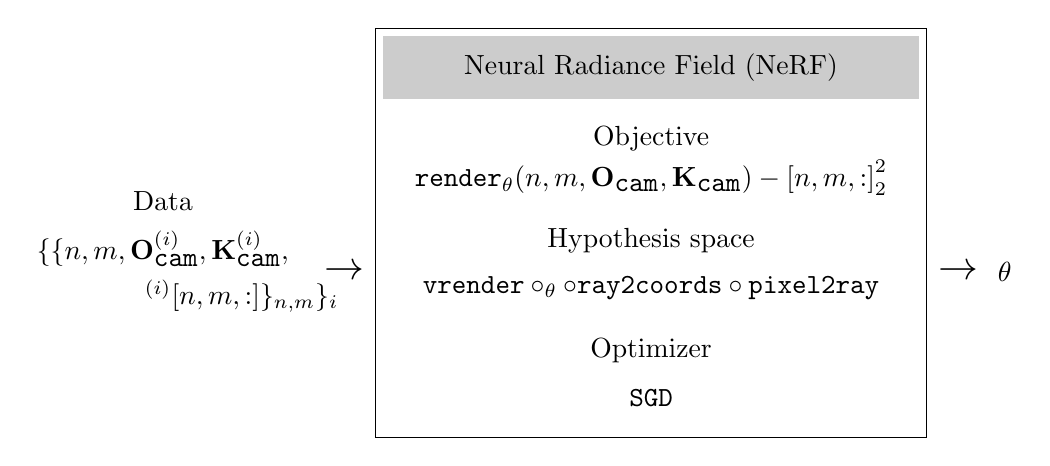
\begin{tikzpicture}
    \draw (0,0) rectangle (7,5.2); % outer box
    \fill[black!20] (0.1,4.3) rectangle (6.9,5.1); % gray box
    \node[] at (3.5,4.7) {{Neural Radiance Field (NeRF)}};
    \node[] at (3.5,3.8) {Objective}; \node[] at (3.5,3.3) {$ \norm{\texttt{render}_{\theta}(n,m, \mathbf{O}_{\texttt{cam}}, \mathbf{K}_{\texttt{cam}})-\boldimg[n,m,:]}_2^2$};
    \node[] at (3.5,2.5) {Hypothesis space}; \node[] at (3.5,1.9) {$\texttt{vrender} \circ \lightfield_{\theta} \circ \texttt{ray2coords} \circ \texttt{pixel2ray}$};
    \node[] at (3.5,1.1) {Optimizer}; \node[] at (3.5,0.5) {\texttt{SGD}};
    \node[] at (-2.7,3) {Data};
    \node[] at (-2.7,2.4) {$\{\{n,m, \mathbf{O}^{(i)}_{\texttt{cam}}, \mathbf{K}^{(i)}_{\texttt{cam}}, $};
    \node[] at (-1.7,1.8) {$\boldimg^{(i)}[n,m,:]\}_{n,m}\}_i$};
    \node[] at (-0.4,2.1) {{\Large  $ \rightarrow$}};
    \node[] at (8,2.1) {{\Large $\lightfield_\theta$}};
    \node[] at (7.4,2.1) {{\Large  $ \rightarrow$}};
\end{tikzpicture}
\end{center}
\marginnote{Fitting a NeRF is very much like solving a magic square puzzle. We try to find the radiance field (the square) that integrates to the observed images (the row and column sums of the square).}[-2.6cm]

%Here is the way NeRF works. First it maps from images to parameters $\theta$ of $F_\theta$ that (implicitly) represents the scene as an RGB$\alpha$ field. Then NeRF renders that field into novel views using volume rendering:
% \begin{figure}[h!]
%     \centering
%     \includegraphics[width=1.0\linewidth]{figures/nerfs/nerf_training_nested_diagram.pdf}
%     \caption{NeRF training. Imags go in, the learner outputs parameters of an MLP that implicitly represents the radiance field. This is unpacked into an explicit representation (the RGB$\alpha$ at each queried point in the 5D field). Finally volume rendering computes a line integral through this field to obtain the color of each pixel (camera ray) in a novel view.}
%     \label{fig:enter-label}
% \end{figure}

From this perspective, NeRF is a clever hypothesis space for constraining the mapping from inputs to outputs of a learned rendering system. Of course we could have used a much less constrained hypothesis space such as a big transformer that directly maps from input pixel coordinates to output colors, without the other modules like $\texttt{ray2coords}$ or $\texttt{vrender}$. However, such an unconstrained approach would be much less sample efficient and require far more data and parameters to learn a good rendering solution (refer back to \chap{\ref{chapter:problem_of_generalization}} to recall why a more constrained hypothesis space can reduce the required amount of training data to find a good solution). However, such a solution could also be more general purpose, as it could handle optical effects that are not well captured by radiance fields.

In fact, there are two products you can get out of a trained NeRF, one for the graphics community and one for the vision community. The graphics product is a system that can render a scene from novel viewpoints. This works by just applying $\texttt{NeRF render}_{\theta}$ (\fig{\ref{fig:nerfs:full_nerf_pipeline}}) to new cameras with new viewpoints. The second product is an inferred radiance field, which tells us something about what is where in the scene. For example, the density of this radiance field can tell us the geometry of the scene, as we will see in the following example of fitting a NeRF to our Flatland scene.

% NeRF maps input rays to output colors. There are a few ways one could do this: (1) computer graphics, (2) machine learning. NeRF does a bit of both. It represents the mapping partially in terms of classical rendering equations and partially in terms of free parameters learned with machine learning. Here is the system. Black lines are classical baked in rendering equations and blue lines are the learned parameters:

% This is often a good strategy. It is much more sample efficient than learning everything. But it only works if we know something about the true mapping. Here we know it is rendering a scene with cameras and light.

\begin{figure}[t]
    \centerline{
    \includegraphics[width=1.0\linewidth]{figures/nerfs/flatland_training.jpg}
    }
    \caption{Iterations of training a NeRF in Flatland. All of these are top-down views of the world (we are looking at Flatland from above, which is a view the inhabitants cannot see). (a) The radiance field visualized as an image with color equal to the color of the field at each position and transparency proportional to the density of the field at each position. (b and c) The volumetric rendering process for two different cameras looking at the radiance field. The circle colors and transparencies again show the color and density of the field, and the circle size shows the $\alpha$ value as we walk along each camera ray. Small circles mean those points are more occluded; i.e. there is a low probability of the ray reaching them and they contribute very little to the volumetric rendering integral.}
    \label{fig:nerfs:flatland_training}
\end{figure}

In \Fig{\ref{fig:nerfs:flatland_training}}, we show several iterations of the fitting process. The top row shows the radiance field as seen from above. This is a perspective our Flatlanders cannot directly see but can infer, just like we on Earth cannot directly see the full shape of a 3D ($X,Y,Z$) radiance field but can infer it from images. The bottom rows show volumetric rendering from two different cameras. The small circles along the rays are samples of the radiance field. Their size is the $\alpha$ value at that location along the ray, and their color and opacity are the color and density values of that location in the radiance field. Notice that initially we have a hazy cloud of stuff in the middle of the scene and over iterations it congeals into solid objects in the shapes of our Flatland denizens. After around 2,500 steps of gradient descent, we have arrive at a fairly accurate representation of the scene. At this point, the objects' densities are high enough that volumetric rendering essentially amounts to just ray casting and finding the color of the first surface we hit. So why did we use volumetric rendering? Not because we care about volumetric effects; in this scene there are none. Rather because it makes it possible for optimization to find the ray casting solution. This is the second, and arguably main, benefit of volumetric rendering that we alluded to previously (the first being the ability to model translucency and subsurface effects).

%Once we have this field represented explicitly, we can render through it. Really we do not need to evaluate $f_\theta$ at all locations. We only need to evaluate along the ray we are rendering. So we sample some points along the ray. This is a discrete approximation to the rendering integral. It looks like this:




\section{Concluding Remarks}

Radiance fields try to model the light content in a scene. The ultimate goal is to model the full plenoptic function, that is, all physical properties of all the photons in the scene. Along the way to this goal, many simplified models have been proposed, and this chapter focused on just one of them: NeRFs. NeRFs combine the ideas of radiance fields and volumetric rendering with topics we have seen earlier, such as multiview geometry, signal processing, and neural networks. They appear near the end of this book because they rest upon almost all the foundations we have by now built up.



